\capitulo{6}{Trabajos relacionados}

Durante la realización de este proyecto, se han tomado referencias de otros trabajos para poder tomar ideas y moldearlas de manera que se genere un producto completo y de calidad. A continuación, se detallan los trabajos y programas de los que se han tomado referencias o que se encuentran relacionados en este ámbito.

\section{Atribuciones de género y construcción de identidades en la literatura infantil sobre prehistoria }

El estudio de Alberto San Martín Zapatero y Delfín Ortega-Sánchez~\cite{san2022atribuciones}, titulado 'Atribuciones de género y construcción de identidades en la literatura infantil sobre prehistoria', examina cómo los libros infantiles dedicados a la prehistoria presentan estereotipos de género. Publicado en el Bellaterra Journal of Teaching \& Learning Language \& Literature, este trabajo utiliza técnicas de análisis de contenido para evaluar textos e ilustraciones, revelando que a menudo se distorsionan los roles de género y se alejan de los últimos avances científicos.

Este proyecto se inspira en este estudio para desarrollar su metodología de análisis. La herramienta del estimador del proyecto evalúa de manera objetiva la presencia de sesgos de género en los libros infantiles, adaptando y ampliando las categorías de análisis propuestas en el estudio de San Martín Zapatero y Ortega-Sánchez.

Ambos trabajos comparten el objetivo de alcanzar un discurso inclusivo en la literatura infantil sobre prehistoria y basado en evidencias científicas, proporcionando recursos educativos que reflejen una visión más justa de la prehistoria. Esta colaboración y adaptación de metodologías refuerza la importancia de revisar y actualizar los materiales educativos para eliminar los estereotipos de género.

\section{Discord}

Discord\footnote{Web de \href{https://discord.com/}{ Discord}} es una red social de comunicación que sido una gran referencia para la parte lógica, ya que se ha tomado como referencia para la lógica de permisos del personal de administración. Esta parte ha sido desarrollada de manera similar, donde en un grupo el administrador puede crear los roles que se necesiten y aplicar unos permisos personalizados para los usuarios con esos roles.

\begin{figure}[h]
\centering
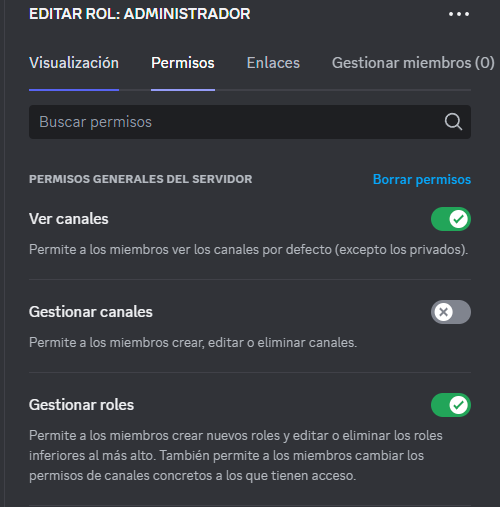
\includegraphics[width=0.6\linewidth]{Imagenes/Discord.png}
\caption{Permisos Discord}
\label{Permisos Discord}
\end{figure}
\FloatBarrier